% Created 2020-05-06 mié 13:50
% Intended LaTeX compiler: pdflatex
\documentclass[a4paper, 12pt]{article}
\usepackage[utf8]{inputenc}
\usepackage[T1]{fontenc}
\usepackage{graphicx}
\usepackage{grffile}
\usepackage{longtable}
\usepackage{wrapfig}
\usepackage{rotating}
\usepackage[normalem]{ulem}
\usepackage{amsmath}
\usepackage{textcomp}
\usepackage{amssymb}
\usepackage{capt-of}
\usepackage{hyperref}
\usepackage{float, amsfonts, commath, mathtools}
\author{Tabaré Pérez}
\date{\today}
\title{Lecture 13 - 8 The K-Means Algorithm: The Specifics}
\hypersetup{
 pdfauthor={Tabaré Pérez},
 pdftitle={Lecture 13 - 8 The K-Means Algorithm: The Specifics},
 pdfkeywords={},
 pdfsubject={},
 pdfcreator={Emacs 26.3 (Org mode 9.3.6)}, 
 pdflang={English}}
\begin{document}

\maketitle
So let's just look at this algorithm.

\begin{enumerate}
\item Randomly select \(z^{(1)} \ldots z^{(K)}\). And we will talk shortly about
different strategies of how to do random initialization. But for now, just
you assume it totally randomly selected them.

\item And then we will iterate over the following two steps:

\begin{enumerate}
\item Given \(z^{(1)} \ldots z^{(K)}\), assigns \(x_s\) to the closest \(z\):
\[\text{cost}(z^{(1)} \ldots z^{(K)})=\sum_{i=1}^{n} \min_{j=1 \ldots K} \norm{x^{(i)} - z^{(j)}}^2\]
\item Given \(C_1 \ldots C_K\), find the best representatives \(z\):
\[\text{cost}(C_1, \ldots ,C_K) = \min_{z^{(i)} \ldots z^{(K)}}\sum_{j=1}^{K}\sum_{i \in C_j} \norm{x^{(i)} - z^{(j)}}^2\]
\end{enumerate}
\end{enumerate}

And there are a few questions that we need to answer here. If you look in the
second step of the algorithm, I am actually telling you exactly how to find the
assignment for every point \(x\): It just will compute its distance to all the
existing \(z\)'s and find the one which is the closest.

Something different happens in this step because in this step, I am just telling
you I want to find the best representative which optimizes this cost, but they
don't really give you a mechanism for doing so.

And what we will do here is what we have done when we were talking about
supervised learning:

We will now look at this objective, take a derivative with respect to variable
we're interested in, making it equal to zero, and it will give us an idea about
the value of the \(z\). So let's be more concrete here.

What we can do here, we can first notice that every cluster selects its
representative independently. So what we would want to do is actually look at a
specific cluster. Let's say we're looking at cluster \(j\) and we're trying to
find \(z\)s, which will minimize this particular sum:

\begin{equation}
C_j: \sum_{i \in C_j} \norm{x^{(i)} - z^{(j)}}
\end{equation}

Our goal is to find the \(z^{(j)}\), which will minimize the sum. So what we
will do, we will take derivative with respect to the \(z\), make it equal to
\(0\), and it will give us an idea about the \(z\).

\begin{equation}
C_j: \frac{\partial}{\partial z^{(j)}} \left[\sum_{i \in C_j} \norm{x^{(i)} - z^{(j)}}\right] = 0
\end{equation}

So we are taking the derivative with respect to the \(z^{(j)}\), making equal to
zero, and then we can find the corresponding \(z^{(j)}\).

You would actually do this computation as your exercise, but I would show you
what is the answer that you're supposed to get. So in this case, what you will
find out is actually quite intuitive. You would find out that this \(z^{(j)}\)
is the centroid of this group. This will be the sum of all \(x^{(i)}\) in this
particular cluster over the size of \(C_j\):

\begin{equation}
z^{(j)} = \frac{\sum_{i \in C_j} x^{(i)}}{\abs{C_j}}
\end{equation}

So what we've got is what one would expect to get. It's just that the
representative would be the point, which is in the center of the cluster. And
now, there is another interesting question is, why do I have to use square
Euclidean distance as part of k-means? And this is exactly the answer to this
question because if you make the derivative and you do the computation, you
would see that your representative have to have this form. However, if you would
have been using here some other distance, not the square Euclidean distance,
this computation will not work out this way, and this is an important point to
understand:

\textbf{This algorithm only works if the distance measures that you're using is square
Euclidean distance}.

And we will talk later about different extensions of how we can enable to expand
this class of algorithm to be able to operate with any distance function.

Now, the next question that you may ask ourselves, you see a road to iterate. So
how many iterations do I actually need to take? How do I know that this
algorithm converges and to what value does this algorithm converges?

So that on the guarantees that we have about this algorithm is that it converges
and it would converge to a \textbf{LOCAL MINIMUM}.

So, first of all, let's think about its convergence. How do we know that it does
converge? Because, what happens here?

\begin{itemize}
\item First of all, our cost function is not negative.
\item Second, we also know that through every single iteration of this algorithm, it
either stays the same,and in this case we can stop, or it decreases.
\end{itemize}

And since the number of partition is finite, we are guaranteed to converge in
this case.

But again, the convergence is \textbf{LOCAL}.

What exactly does it mean?

It means that if you start with a different initialization, you may get a very
different partitioning. And to demonstrate to you how bad it could go, I would
give you a very contrived example. And in this case, this is how bad
initialization may impact your performance. Let's look at the impact of
initialization.

Impact of initialization:

\begin{figure}[H]
\centering
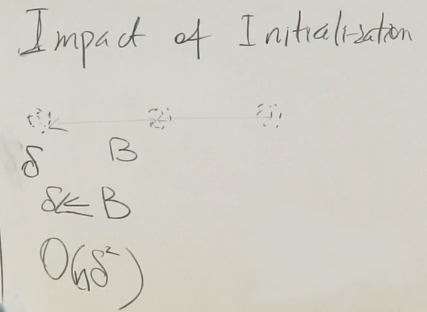
\includegraphics[width=0.5\textwidth]{./pic/04-08-fig-01.png}
\caption{\label{fig:orgfe450b6}Impact of initialization}
\end{figure}

So I will give you this scenario where the answer to you would be very clear.

I would assume that I have naturally, this is the input to my algorithms, three
clusters.

So we will have three clusters, three balls of points, and they will be tiny.
They would have a radius of \(\delta\).

But, obviously, the algorithm doesn't know it has to uncover them.

But these balls would be very much separated from each other. The distance
between these balls is going to be some \(B\). And we know that \(\delta\) is
orders of magnitude smaller than \(B\).

So the clusters are tiny, the distance between these balls is very large.

Now let's think about the following question. If we did a good job and if we
really computed these balls to be the way I drew them, those will be the three
clusters. You can imagine the centroid will be somewhere in the middle of each
cluster.

And the cost that you're going to be encountering would be something in the
order of magnitude of \(\mathcal{O}(\delta^{2})\) because you look at the square
distance between the center and every point. Something of that nature, correct?
And multiply, because we have \(n\) points, it would be
\(\mathcal{O}(n\delta^{2})\).

Now, see what happens if I'm going to do bad initialization. And the bad
initialization I'm going to do will be the following:

\begin{figure}[H]
\centering
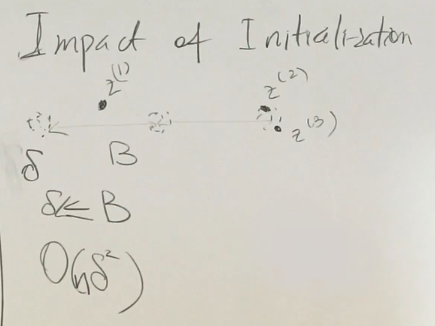
\includegraphics[width=0.5\textwidth]{./pic/04-08-fig-02.png}
\caption{\label{fig:org0d546c2}Impact of initialization}
\end{figure}

The first sets that I'm going to find is going to be here. And the second is
going to be here and the set are going to be located here. So let's call them
\(z^{(1)}\), \(z^{(2)}\), and \(z^{(3)}\).

Let's see how do they behave. So now, after I put this initialization, what will
happen? Points in the first two clusters are pretty happy because they would be
close to this center (\(z^{(1)}\)) and they would stay here and not move.

Now, points here (the third cluster) are going to move according to where do
they lie with respect to \(z^{(2)}\) and \(z^{(3)}\).

Pretty much you're going to take the third ball and split it into two balls,
correct?

Let's look at the next step. During the next step, what will happen? These
points (first cluster) are happy. This centroid, \(z^{(1)}\) is exactly in the
middle. They're not going to move. They're staying there and their
representative is in place. Everybody happy. No movement happens there.

Here, at some point, at least, this point, \(z^{(2)}\) and \(z^{(3)}\) would be
somewhere located in the third tied ball. And then everybody are happy. They
don't want to move out. These two are controlling the points in this cluster and
this guy, \(z^{(1)}\), is controlling these two clusters.

So in this case, the distance between these points to their centroids, as we
said, it's something proportional to B, is going to be really, really high
number.

So overall, the cost of this clustering would be something in the order of
magnitude of \(\mathcal{O}(nB^2)\). And as I said earlies, \(B\) is
substantially larger than \(\delta\).

So in this case, because you started in the wrong place, your algorithm
converges to very suboptimal solution with a very high cost.

So what this example illustrates to you that depending how you start, you may
end up in a very unsuccessful clustering.

And again, looking at this example, we can see what is the problem:

The problem here is that when we decided, when we randomly initialized it, we
put points which are very close to each other (\(z^{(2)}\) and \(z^{(3)}\)). We
put two centroids which are very close to each other.

So maybe one intuition from here is that if we randomly initialize our centers,
we actually may want to spread them around rather than put them closer together.

And there are algorithms which capture this intuition and provide you a
mechanism for selecting this random initialization, which results in a better
theoretical guarantees.

But when you are practically trying to do it, you may want to try your
clustering with several initialization and see what kind of result does it
produce for you.

So at this point, we've already have seen the k-means algorithm, we've seen the
convergence properties of this algorithm, and we also realize an important
drawback of this algorithm, that it's very sensitive to initialization.

And we understood how the properties of initialization will be impacting the
final results.

So with that, we completed the discussion on k-means algorithm.
\end{document}